\section{Comparaison avec la photo d'une rotation de
$90^{\circ}$}\label{comparaison-avec-la-photo-dune-rotation-de-90circ}

\begin{figure}[htbp]
\centering
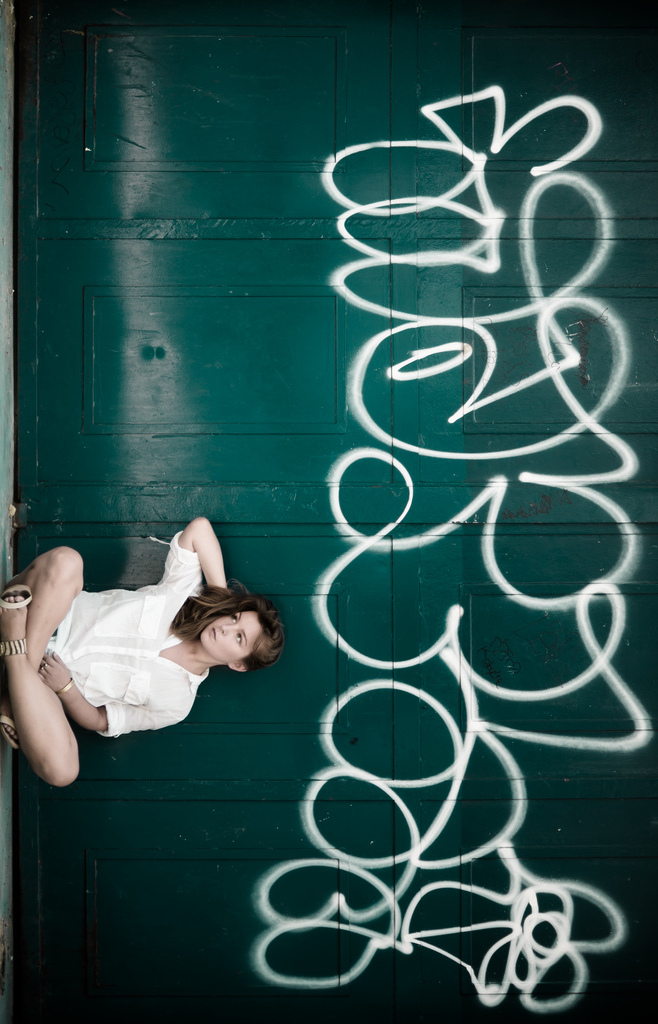
\includegraphics[scale=0.43]{../../photos/rotation.jpg}
\caption{Photo rotation $90^{\circ}$}
\end{figure}

\begin{table}[htbp]
\centering
\begin{tabular}{llr}
\bfseries Formes &
\bfseries Bhattacharyya (\%)%
\DTLforeach*[\DTLiseq{\fichier}{photos/rotation.jpg}]{valeurs}{%
\fichier=Fichier, \formes=Formes,\bhatta=Bhattacharyya, \hue=Hue, \saturation=Saturation, \value=Value}{%
\\
\formes & \bhatta}
\end{tabular}
\end{table}

Contrairement à la photo précédente, cette rotation de $90^{\circ}$ ne
découpe pas l'text = Image donc la différence de couleur est encore plus faible
($0.04 \%$) alors que la différence de forme augmente encore ($58.03 \%$).